
\chapter{\label{cha:intro}Introduction}

\section{Motivation}


\subsection{Research questions}

The main research question is the following:

\textbf{How to facilitate the work of scientists and organizations interested in user modeling and analysis?}\\

The following sub-questions articulate the problem:

\begin{enumerate}
\item \textbf{How to enable users to add custom functionality and change system's behaviour?} (plug-ins)

\item \textbf{Is it possible to develop a component that enables users to store and retrieve information in arbitrary data formats?} (Universal datastore)

\item \textbf{How to enable users to maintain their results up-to-date?}  (Scheduling)


\item \textbf{How to enable multiple users to use the system simultaneously without interfering with each other and keeping their work and results protected?} (Multi User and privacy)


\item \textbf{How can real-world use cases benefit from this system?}

\end{enumerate}

\subsection{Contributions}

\subsection{Organization of the work}

There are many possible ways to approach that. One can use the waterflow model, incremental, ....

In this work we will use the incremental model because of the many advantages it brings. We design and implement one feature at a time, providing a working system after each iteration.

The last thing that has to be considered before launching the next phases of the project is to decide on the order in which the features will be implemented. This issue is addressed in the next section.

\begin{figure}[h!]
  \centering
      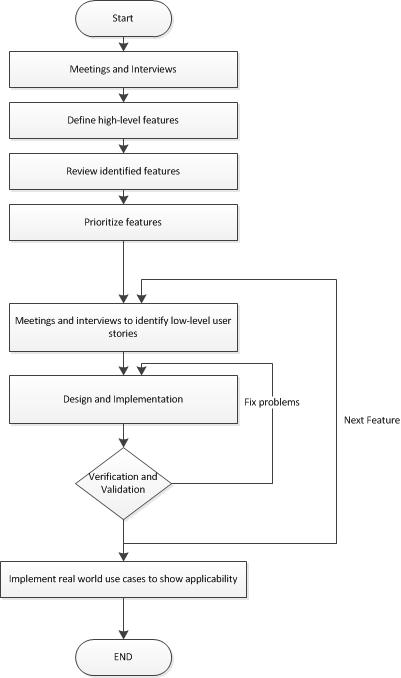
\includegraphics{introduction/WorkOrganization.jpg}
  \caption{Flow chart defining the sequence of actions taken in order to complete the project.}
\end{figure}

\subsection{Organization of the thesis}


